%% LyX 2.0.6 created this file.  For more info, see http://www.lyx.org/.
%% Do not edit unless you really know what you are doing.
\documentclass{article}
\usepackage[latin9]{inputenc}
\setlength{\parskip}{\medskipamount}
\setlength{\parindent}{0pt}
\usepackage{amsmath}
\usepackage{amssymb}
\usepackage{tikz}
\makeatletter
%%%%%%%%%%%%%%%%%%%%%%%%%%%%%% User specified LaTeX commands.

%
\usepackage{amsfonts}\usepackage{nopageno}%%%  The following few lines affect the margin sizes. 
\usepackage{pgfplots}
\pgfplotsset{compat=1.6}

\pgfplotsset{soldot/.style={color=blue,only marks,mark=*}} \pgfplotsset{holdot/.style={color=blue,fill=white,only marks,mark=*}}

\addtolength{\topmargin}{-.5in}
\setlength{\textwidth}{6in}       
\setlength{\oddsidemargin}{.25in}              
\setlength{\evensidemargin}{.25in}         
  
\setlength{\textheight}{9in}
\renewcommand{\baselinestretch}{1}
\reversemarginpar   
%
%

\makeatother

\begin{document}

\title{STA 6326 Homework 4 Solutions}


\author{Maksim Levental}


\date{\today}
\maketitle
\begin{enumerate}
\item [4.1]

\begin{enumerate}
\item Probability of falling within the unit circle is area of the circle
divided by area of $\Omega$. Hence $P\left(X^{2}+Y^{2}<1\right)=\pi/4$.
\item $P\left(2X>Y\right)$is the area below the line $y=2x$, divided by
the area of $\Omega$. The portion of quadrant one that's above the
line is the same as the portion in quadrant 3 that's below the line,
and all of quadrant 4 is included. Hence $P(2X>Y)=1/2$.
\item 

\begin{tikzpicture}
%graph
\draw[draw=gray!50!white,fill=gray!50!white] 
    plot[smooth,samples=100,domain=-1:1] (\x,{-1}) --
    plot[smooth,samples=100,domain=-1:1] (\x,{1});
% \draw[domain=0:4] plot (\x,{1});
% \draw[samples=100,domain=.25:4] plot (\x,{ln(\x)}) node[above left]{$y=\ln x$};
%coordinate grid
\draw (-.5,0)--(4.5,0) node[right]{$x$};
\draw (0,-1.5)--(0,2.5) node[above]{$y$};
\foreach \x in {1,2,3,4}
    \draw (\x,2pt)--(\x,-2pt) node[below] {$\x$};
\foreach \y/\ytext in {1,2}
    \draw (2pt,\y)--(-2pt,\y) node[left] {$\y$};    
%labels 
\node at (.75,.5) {$\mathcal{D}$};
\end{tikzpicture}

\end{enumerate}
\end{enumerate}

\end{document}
